\documentclass[a4paper, 11pt]{article}

\usepackage[english]{babel}
\usepackage[utf8x]{inputenc}
\usepackage{amsmath}
\usepackage{amssymb}
\usepackage{float}
\usepackage{graphicx}
\usepackage[colorinlistoftodos]{todonotes}
\usepackage[authoryear]{natbib}
\usepackage{hyperref}
\usepackage{authblk}
\usepackage[margin=1in]{geometry}
\usepackage{pgfplots}
\pgfplotsset{compat=1.12}
\usepackage{biblatex} %Imports biblatex package
\addbibresource{Bibliography.bib} %Import the bibliography file
\renewcommand{\baselinestretch}{1.2}

\usepackage[inline,ignoremode]{trackchanges} % Documentation of this package can be found at http://trackchanges.sourceforge.net/
\addeditor{MWS} % For each editor, repeat this command with their initials. Monroe is added by default.


\title{\vspace{-1cm}COVID-19 Prediction from Symptoms}
\author{Guankai Zhai, Weiyan Wu, Jianyang Zhou}
\date{\today} % You can write in any date within the brackets.

\begin{document}

\maketitle

\begin{abstract}
Since 2020, the COVID-19 pandemic has affected the world in different aspects and infected thousands of people. Patients with COVID-19 infections have different clinical symptoms and outcomes. In this project, we used different machine learning models to explore the relationship between different symptoms and whether the patients are tested positive for COVID-19. \par
Specifically, we cleaned our data set and conducted some exploratory data analysis (EDA) to determine which symptoms are highly linked to a positive diagnosis of COVID-19. Then we fitted several classification models on this dataset and compared their performance metrics with respect to different hyperparameters. Finally, we analyzed the differences in symptoms between COVID-19 and influenza. 



\end{abstract}
\section*{Introduction}
As the world began to mount an unprecedented worldwide response to COVID-19 in early 2020, it lacked a standardized, global way to measure COVID-19 illness and track the pandemic that would help guide decision-making (e.g., implementation of social distancing measures). One approach to quickly classifying patients as COVID-19 positive or negative could be through machine learning algorithms. While the use of machine learning has been applied to contact tracing and forecasting during the COVID-19 epidemic, it has only limitedly been explored as a means for accurately predicting COVID-19 infection on clinical presentation. \par 

With just a few important parameters clinicians can diagnose the patients well before a laboratory diagnosis. We believe that machine learning could achieve a similar level of competence. There remains a paucity in research showing the capacity of machine learning algorithms in identifying COVID-19 patients and differentiating between COVID-19 and influenza patients. \par

Thus, a model to identify infected patients from the symptoms they display is urgently needed. The Israeli Ministry of Health publicly released data of all individuals who were tested for SARS-CoV-2 via RT-PCR assay of a nasopharyngeal swab \cite{data}. We leveraged this data to build a classifier which, given a patient's indicated symptoms, could classify the patient as either being infected or not.


\section*{Data Cleaning and Preparation}
We first imported the dataset into a Jupyter Notebook. The dataset contains 7,651,053 observations each with 10 dimensions. With one dimension being the date of the test, 8(cough, fever, sore throat, breath shortness, headache, age 60 and above, gender, and test result) of the remaining 9 dimensions are binary variables and 1(test indication) has three categories. \par
We then drop corrupt observations(i.e contain NaN values). After this, we are left with 597,7416 entries. With some of the data being in Hebrew, we used the GoogleTrans API to translate these entries into English for better interpretability. We also changed categorical variables with string representations into 0s and 1s. \par
The dataset is highly unbalanced, with around $90\%$ of the observations having a negative COVID result and the rest being positive. We thus trimmed our dataset so that we have a 50-50 split of positive and negative cases. After this step, we still have around 1,000,000 observations left, which is sufficient for the training and testing of our models.
Finally, we used one-hot encoding to encode the dimension of "test indication", which could be "Contact traced," "Abroad," or "Other."

\section*{Exploratory Data Analysis}
We then began to conduct some exploratory analysis on our data to determine what is relevant with the test result.
We start by plotting the number of positive cases over time. \par
\begin{figure}[H]
\centering
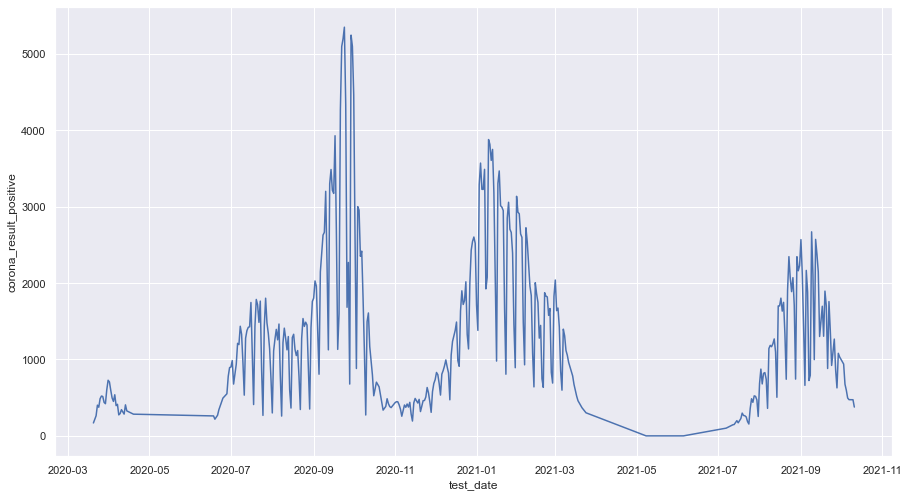
\includegraphics[scale=0.4]{total.png}
\caption{Total Number of Positive Cases with Time.}
\label{Confirmed Cases}
\end{figure}
Despite the daily differences that make the graph non-continuous, We find that the number of positive cases varies with time and that the pandemic comes in the form of waves: the number of total positive cases would increase up until a certain point, after which it started to go down. This cycle has repeated several times since the onset of this pandemic. Thus, we believe that warnings about upcoming waves are essential for policy making and supply chain preparations, which will be discussed in greater detail in the last section of this report. \par
We then start exploring factors that change the probability of the tests being positive. Intuitively, the patient having any of the listed symptoms would mean that his/her test is more likely to be positive. We summarize the statistical results below after separately computing the mean rates of positive cases when each symptom/feature is present and not.\par
\begin{table}[H]
\centering
\caption{Percentage of Positive Tests Given a Symptom}
\begin{tabular}{| l | c | c | c | c | c |}
\hline
Symptom & Cough & Fever & Sore Throat & Shortness of Breath & Headache  \\ \hline
w/o Symptom & 7.2 & 7.3 & 7.9 & 8.4 & 7.2 \\ \hline
w/ Symptom & 37.9 & 41.8 & 43.0 & 51.2 & 43.5 \\
\hline
\end{tabular}
\label{Table}
\end{table}

We then start to explore the relationship between the proportion of positive cases and the other characteristics, which is even more interesting. We tabulate our results below, in a similar fashion to the last part.
\begin{table}[H]
\centering
\caption{Percentage of Positive Tests Given a Characteristic}
\begin{tabular}{| l | c | c | c | c |}
\hline
Characteristic & Being Male & $Age \ge 60$ & Being Abroad & Contact Traced  \\ \hline
w/o Characteristic & 8.8 & 8.7 & 8.6 & 5.4 \\ \hline
w/ Characteristic & 8.3 & 8.1 & 11.2 & 43.9 \\
\hline
\end{tabular}
\label{Table}
\end{table}

Finally, to illustrate the correlation between different variables in an intuitive manner, we plot the following heatmap of the correlation matrix.
\begin{figure}[H]
\centering
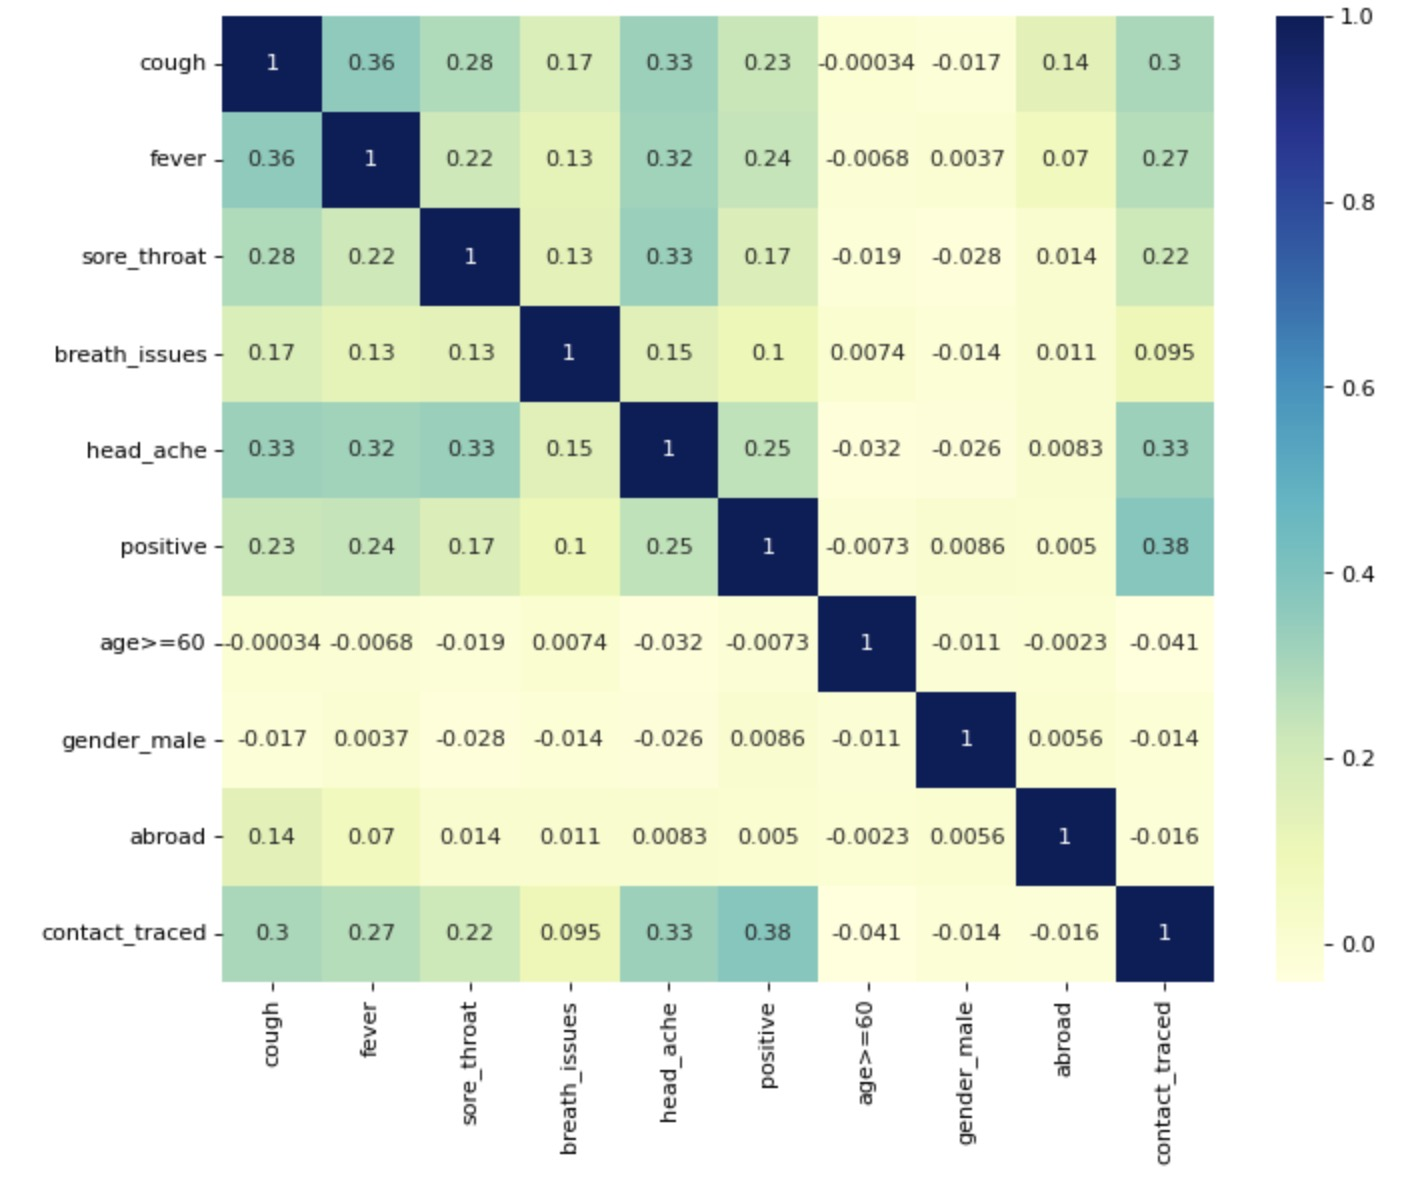
\includegraphics[scale=0.23]{heatmap.jpg}
\caption{Correlation Heatmap of Our Dataset.}
\label{heatmap}
\end{figure}

This heatmap confirms our previous statistics tables. As it could be seen, all variables except "age$\geq$60", "gender\_male", and "abroad" have a significant correlation factor with the target variable "positive". \par
Another interesting observation is that many of the symptoms are also highly correlated, such as cough and fever. This could potentially hinder the effectiveness of our models, but since we are also concerned with diagnosing between COVID-19 and influenza (the second part of this project), we will leave this for now.

\section*{Models}
Given the above exploratory analysis, we can conclude that all symptoms in the dataset as well as some characteristics(Being Abroad and Contact Traced) have an impact on the chance that a test is positive. We thus include these as our features. We did not include the other non-important features to prevent overfitting. We choose the test results (either 1 or 0) as our labels. We then separated our data into training and testing datasets. Since the original dataset is large, we only used $0.5\%$ of our data for validation, which is around 5000 observations and should give us a very accurate estimate of our models' performance according to the Central Limit Theorem. \par
To evaluate the performance of our models, we will look at the overall k-cross-validated accuracy as well as the false-positive and false-negative rates. We will also look at the receiver operating characteristic (ROC) curves, which plot the True Positive Rate against the False Positive Rate, where applicable. Since testing a patient is not particularly expensive but missing an infected patient has a large negative externality, we prefer a small false negative rate and are willing to accept a relatively high false positive rate. \par
Since we excluded features that are shown to have little impact on the positive rate and our sample size is relatively large, we believe that overfitting is not very likely.

\subsection*{Logistic Regression}
We first build a classifier with Logistic Regression. The reason we use this as our first model is that logistic regression inherently yields the probabilities of each label, which is very helpful if we want to control our false positive/negative rate. However, the accuracy of this model, at $76\%$ after cross-validation, is not particularly impressive.\par
However, if we decrease our threshold of positive to 0.2 (i.e. any patient whose probability of being positive is greater than 0.3 will be classified as positive), our false negative rate will decrease to 0.15, which is satisfactory. As the following diagram shows, an even lower false-negative rate (FNR) could be achieved at the expense of a higher false-positive rate(FPR).\par
\begin{figure}[H]
\centering
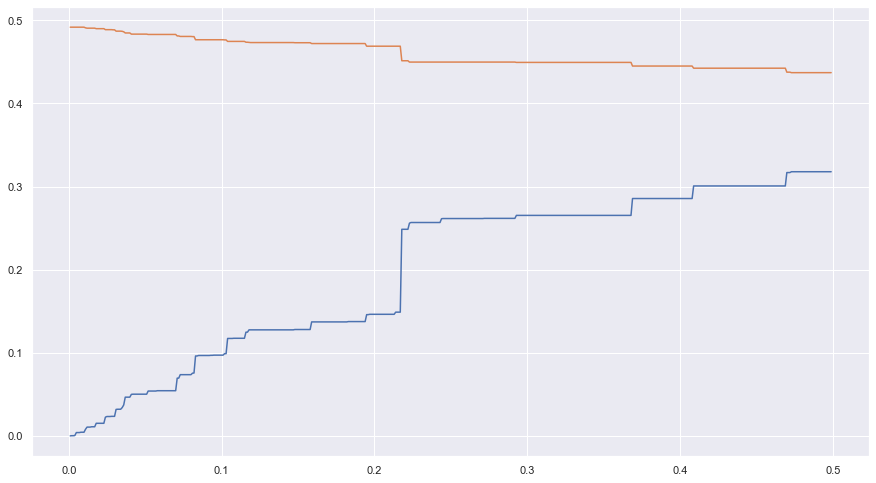
\includegraphics[scale=0.4]{fps.png}
\caption{FPR(Orange) and FNR(Blue) with Decision Threshold.}
\label{Confirmed Cases}
\end{figure}

\subsection*{K-Nearest Neighbors}
We then try to build our classifier with the k-Nearest Neighbors Algorithm. The central assumption here is that patients with similar features would have the same label. This is a reasonable assumption to make in our case, despite the similar symptoms between COVID-19 and influenza, which will be discussed below.\par
k-NN has an important hyperparameter: the number of neighbors that we will look at. We tuned this parameter using grid search and plotted the accuracy of each k value in the following graph.
\begin{figure}[H]
\centering
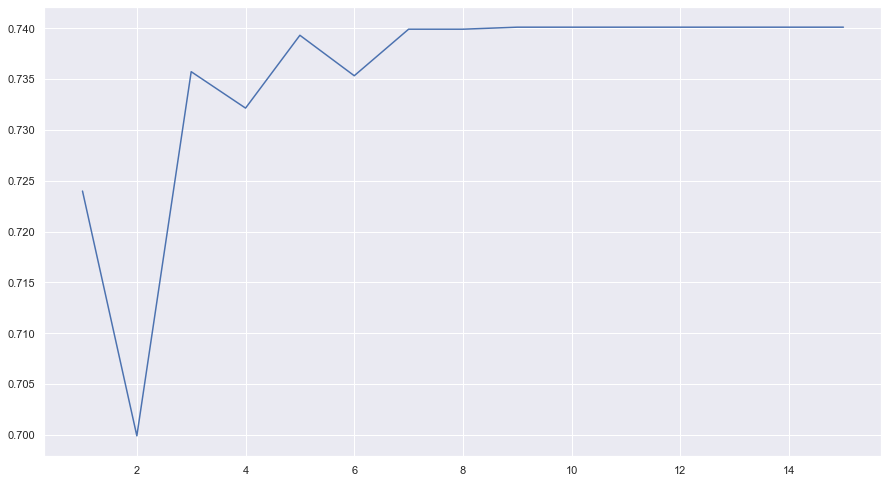
\includegraphics[scale=0.4]{knn.png}
\caption{Accuracy of kNN with Different Values of k.}
\label{Confirmed Cases}
\end{figure}
As it could be seen, the performance of our k-NN algorithm is not that better compared to the above logistic regression. However, the running time of this model was significantly higher than logistic regression during tests, despite having a shorter training time. Thus, this model is inappropriate for our situation in which we will run the fitted model many times for many patients.

\subsection*{Gradient-boosted Decision Trees}
We then try to build our classifier with the Gradient-boosted Decision Trees(GBDT). This is the most common classifier used in industry and is widely known for its accuracy and unlikeliness to overfit. The central idea behind GBDT is that it builds an ensemble of decision trees that each tries to predict the error of its successors. \par
We used a random search to determine the optimal set of hyperparameters for this model. We then measured the accuracy at this model at 80\%, an improvement from the previous two models but still not quite satisfying. 

\subsection*{Analysis of Models}
After running the three models above, it is obvious that our data likely has a high Bayes Optimal Error, which is the error that is given by the best possible classifier had we known the true distribution of the data. GBDT has a relatively high overall accuracy rate, but it is not very flexible during deployment since its false positive and false negative rate could not be easily adjusted. k-NN and Logistic Regression offer similar accuracies, but the former takes a relatively long time during deployment, especially as the data size gets large. We thus believe that Logistic Regression is the best classifier for the above task.
The relatively high Bayes Optimal Error is likely due to the similar symptoms presented by COVID-19 and influenza. In the following section, we try to present a solution to this issue.

\section*{COVID-19 vs Influenza}
As has been mentioned above multiple times, the differentiation between COVID-19 and influenza, a major limit on the accuracy of our current models, is an important task that we need to solve. However, our current dataset is limited in that its features are mostly binary and not continuous. For example, body temperature, which is represented in our dataset as a binary variable(fever), could have been any positive real number, as measured by the physician on a clinical basis. After researching on existing literature and consulting the course staff, we decide to utilize another dataset, provided by the West Virginia University Hospital that preserves more detailed data about 3,884 patients, to accomplish this task \cite{influenza}. A summary of the data is presented in the table below.

\begin{table}[H]
\centering
\caption{Outcomes of WVU patients presented}
\begin{tabular}{| l | c | c | c | c |}
\hline
Category & Overall & COVID-19 Positive & Influenza Positive  \\ \hline
Total & 3883 & 747 & 1223  \\ \hline
No. of ICU Admissions & 655 & 142 & 70  \\ \hline
No. of Patients on Ventilators & 264 & 43 & 39  \\ \hline
No. of Deaths & 261 & 51 & 51  \\ 
\hline
\end{tabular}
\label{Table}
\end{table}

The dataset contains 3883 observations. There are 8 features, including race and ethnicity (categorical), body temperature at admission (continuous positive number), sex (binary between male and female), systolic blood pressure (continuous positive number), diastolic blood pressure (continuous positive number), heart rate (positive real number), oxygen saturation (positive real number), and respiratory rate (positive real number). The results of influenza and COVID-19 tests are both recorded in the dataset. \par
After dropping the NaN values, we are left with around 3500 observations that are sufficient for our purposes. We used one-hot encoding for the categorical variables and also normalized our dataset using min-max scaling, similar to what we did for the first dataset. We split our data into training and testing sets according to the 80-20 proportion.\par


\subsection*{Gradient Boosted Decision Trees}

We first used a Gradient Boosted Decision Tree (GBDT) to predict the data. Instead of using the implementation in Scikit-Learn, we used the XGBoost package this time. The main reason for this choice is the shorter training time while using XGBoost and the extra flexibility that XGBoost offers compared to Scikit-Learn. XGBoost allows us to vary the probability threshold used during testing so that we could manipulate our false positive and false negative rates. \par 
As this is a three-class (COVID-19, influenza, or none) classification problem, we used one-hot encoding for our target variables. After using random search to find the optimal set of hyperparameters, we achieved an accuracy rate of 88\%, which is satisfactory given the limited amount of data we have and a potentially high Bayes Optimal Error. The ROC curve plotted below illustrates the performance of this model.

\begin{figure}[H]
\centering
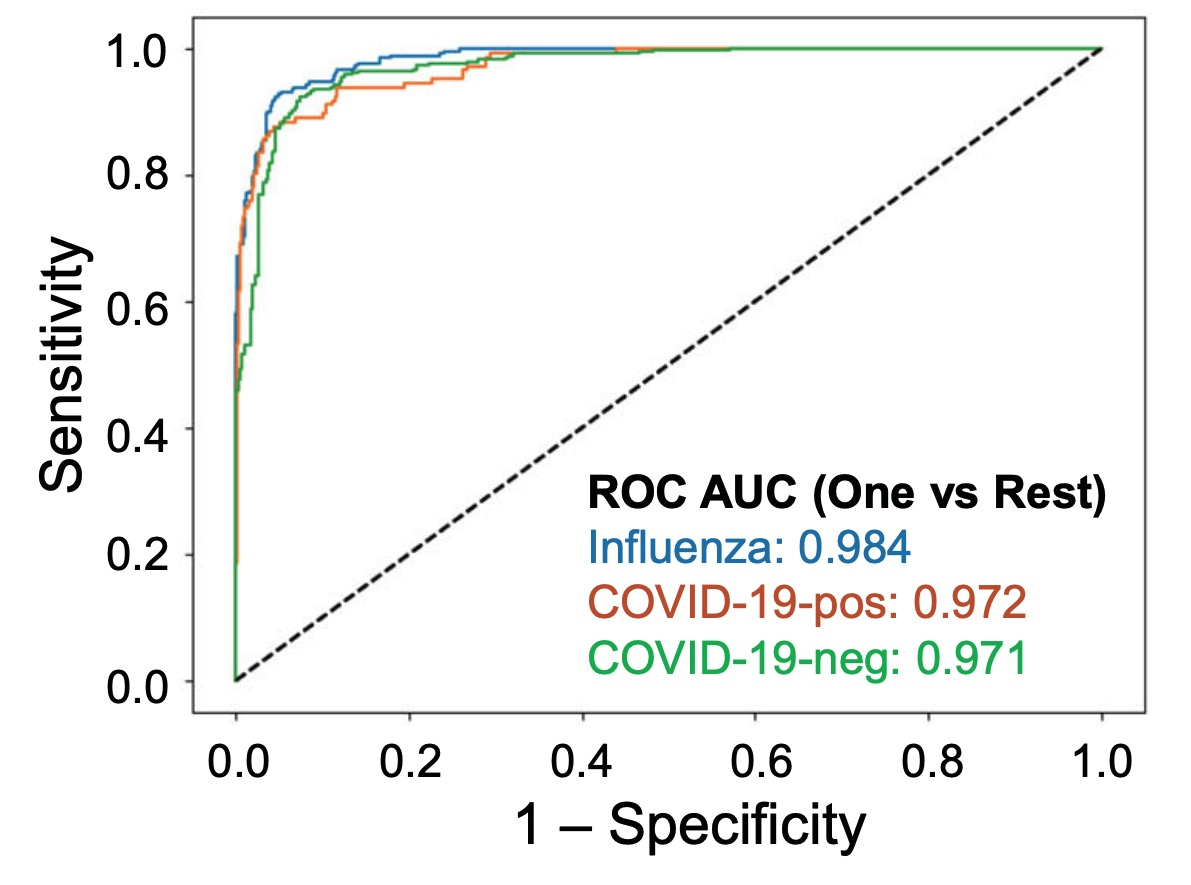
\includegraphics[scale=0.25]{roc.png}
\caption{Receiver Operating Characteristic (ROC) Curve of the GBDT Classifier.}
\label{Confirmed Cases}
\end{figure}

In this figure, the sensitivity is the true positive rate divided by the true positive rate plus the false negative rate. Specificity is the true negative rate divided by the true negative rate plus the false positive rate. As we vary the decision threshold during test time, these two values change together with each other. The area under this curve is what we use to evaluate our classifier. At about 97\% and higher, our classifier is very effective in distinguishing between COVID-19, influenza, and others.

\section*{Conclusion}
In this study, we experimented with several different models and evaluated their performances to shed light on the potential of machine learning algorithms in helping physicians and doctors identify COVID-19 as well as distinguishing it from influenza. \par
However, we still believe that this model should not be used alone and should be supplemented by actual COVID-19 nucleic acid tests. At an accuracy of around 80\% and a false negative rate of around 95\%, using this model solely would impose severe public health risks to the environment. Nevertheless, this model could be used as soon as a patient finishes his/her preliminary clinical tests to determine his/her probability of having contracted COVID. In this way, more medical resources could be mobilized in an efficient manner before the nucleic acid results become available.

\subsection*{Weapon of Mathematical Destruction}
We believe that our models do not constitute weapons of mathematical destruction, since their accuracy rates could be easily measured by clinical nucleic acid tests of COVID-19. While it does have significant negative consequences if its accuracy is not satisfactory and might lead the local area's public health situation into a vicious cycle, its effects could be quickly measured and thus prevented from spreading further.

\subsection*{Fairness Considerations}
Fairness is indeed an important consideration that we have to consider. This is because if the model is biased toward people of a certain characteristic (e.g. white people against black people), this might potentially lead to social injustice and thus negative externalities. One metric that we could utilize to evaluate the fairness of our algorithms is the concept of equalized odds. Specifically, we measure the true positive, true negative, false positive, and false negative rates of our model for people of different races. Our model is fair under this concept if and only if all these metrics are the same for people of different ethnic groups. We thus conducted a chi-square hypothesis test with the null assumption that our model is fair. The p-value of our test is around 35\%. We thus fail to reject our null hypothesis, and our model is indeed fair under this concept of equalized odds.

% \section*{Future Work}
% Given the limited time available for this part of the project, some work remains to be done. This includes but is not limited to the following points.
% \begin{itemize}
%   \item Further analyses on more models for the above prediction challenge. Several possiblities include trees and random forests,  support vector machines, etc. Discussions on the recall and precision rates could also be added.
%   \item A warning system should be built to give alerts about upcoming waves of the pandemic in advance. To achieve this, we plan on integrating the dataset of the daily number of confirmed COVID cases in Israel into our current data. We will then build a regression model to predict the number of cases that will be confirmed in the coming week based on information of the past week.
%   \item A major limitation currently is that COVID-19 patients display very similar symptoms to influenza patients, making prediction difficult. We thus plan to build a Deep Neural Network (with its final layer using the softmax function as activation) to classify patients as either having COVID-19, influenza, or neither. This also requires us to collect an additional dataset that contains this information.
% \end{itemize}

\newpage

\printbibliography


\end{document}

